%2multibyte Version: 5.50.0.2890 CodePage: 65001

\documentclass[12pt]{article}
%%%%%%%%%%%%%%%%%%%%%%%%%%%%%%%%%%%%%%%%%%%%%%%%%%%%%%%%%%%%%%%%%%%%%%%%%%%%%%%%%%%%%%%%%%%%%%%%%%%%%%%%%%%%%%%%%%%%%%%%%%%%%%%%%%%%%%%%%%%%%%%%%%%%%%%%%%%%%%%%%%%%%%%%%%%%%%%%%%%%%%%%%%%%%%%%%%%%%%%%%%%%%%%%%%%%%%%%%%%%%%%%%%%%%%%%%%%%%%%%%%%%%%%%%%%%
\usepackage[onehalfspacing]{setspace}
\usepackage{rotating}
\usepackage{geometry}
\usepackage{caption}
\usepackage{lscape}
\usepackage{epstopdf}
\usepackage{graphicx}
\usepackage[fleqn]{amsmath}
\usepackage{adjustbox}
\usepackage{tabularx}
\usepackage{lipsum}

%TCIDATA{OutputFilter=LATEX.DLL}
%TCIDATA{Version=5.50.0.2890}
%TCIDATA{Codepage=65001}
%TCIDATA{<META NAME="SaveForMode" CONTENT="1">}
%TCIDATA{BibliographyScheme=Manual}
%TCIDATA{Created=Tuesday, February 18, 2014 11:22:17}
%TCIDATA{LastRevised=Thursday, July 21, 2016 10:34:04}
%TCIDATA{<META NAME="GraphicsSave" CONTENT="32">}
%TCIDATA{<META NAME="DocumentShell" CONTENT="Standard LaTeX\Blank - Standard LaTeX Article">}
%TCIDATA{Language=American English}
%TCIDATA{CSTFile=40 LaTeX article.cst}

\geometry{
 a4paper,
 total={210mm,297mm},
 left=27mm,
 right=27mm,
 top=27mm,
 bottom=27mm,
 }
\newtheorem{theorem}{Theorem}
\newtheorem{acknowledgement}[theorem]{Acknowledgement}
\newtheorem{algorithm}[theorem]{Algorithm}
\newtheorem{axiom}[theorem]{Axiom}
\newtheorem{case}[theorem]{Case}
\newtheorem{claim}[theorem]{Claim}
\newtheorem{conclusion}[theorem]{Conclusion}
\newtheorem{condition}[theorem]{Condition}
\newtheorem{conjecture}[theorem]{Conjecture}
\newtheorem{corollary}[theorem]{Corollary}
\newtheorem{criterion}[theorem]{Criterion}
\newtheorem{definition}[theorem]{Definition}
\newtheorem{example}[theorem]{Example}
\newtheorem{exercise}[theorem]{Exercise}
\newtheorem{lemma}[theorem]{Lemma}
\newtheorem{notation}[theorem]{Notation}
\newtheorem{problem}[theorem]{Problem}
\newtheorem{proposition}[theorem]{Proposition}
\newtheorem{remark}[theorem]{Remark}
\newtheorem{solution}[theorem]{Solution}
\newtheorem{summary}[theorem]{Summary}
\newenvironment{proof}[1][Proof]{\noindent \textbf{#1.} }{\  \rule{0.5em}{0.5em}}
\input{tcilatex}
\begin{document}

\title{Business cycle and the persistence on wage dynamics}
\author{ P. Cerqueira\thanks{%
University of Coimbra and GEMF}, N. Luu\thanks{%
University of Coimbra and Minho}, M. Portela\thanks{%
University of Minho and NIPE, and IZA Bonn}, S. Sousa\thanks{%
University of Minho and NIPE. Corresponding author: ssousa@eeg.uminho.pt.} \\
%EndAName
\textit{Preliminary version: please do not quote}}
\maketitle

\begin{abstract}
\singlespacing {\small The recent economic crisis has recalled the researchers' attention to the importance of external economic
 factors not only for the performance of labour markets but for the development of societies in general. The present
paper aims at contributing to the knowledge of the impacts of the business cycle in Portugal, proposing to provide
new insights on  the impact of external conditions at the time of labour market entry on the individual's 
labour market performance. 
Stating by a brief review of the results found in the literature the first contribution of this 
article is to establish the Portuguese business cycle, based on OECD data, from 1970 until 2012.  The relation
between the business cycle and the  impact of entering the labour market in 
 a boom versus in a recession, on individuals' labour market outcome (wage level and persistence) is investigated, based on data from ``Quadros de Pessoal''. 
The results suggest that external economic conditions matter.}
\end{abstract}

%%\date{March 2015}
%%\today

\textbf{Keywords: }Business cycle, LEED, wage persistence

\textbf{JEL Classification:}\textit{\ }C33,\textbf{\ }E32, J31

\section{Introduction}

\lipsum


\begin{center}
\begin{table}[th]
\caption{Descriptive statistics}
\label{tab.r1}
\center  
\scalebox{1.0}{
{
\def\sym#1{\ifmmode^{#1}\else\(^{#1}\)\fi}
\begin{tabular}{l*{1}{ccccc}}
\hline\hline
                    &       count&        mean&          sd&         min&         max\\
\hline
wage                &          49&    2950,271&    1341,222&    1277,173&    7198,693\\
educ                &          49&    8,816067&    3,354241&    3,376724&    18,15874\\
exper               &          49&    19,38776&    6,415529&          10&          29\\
\hline\hline
\multicolumn{6}{l}{\footnotesize Source: own computations.}\\
\end{tabular}
}
%
}
\end{table}
\end{center}

In table \ref{tab.r1} we discuss...

\lipsum

\begin{figure}[!htb]
\centering
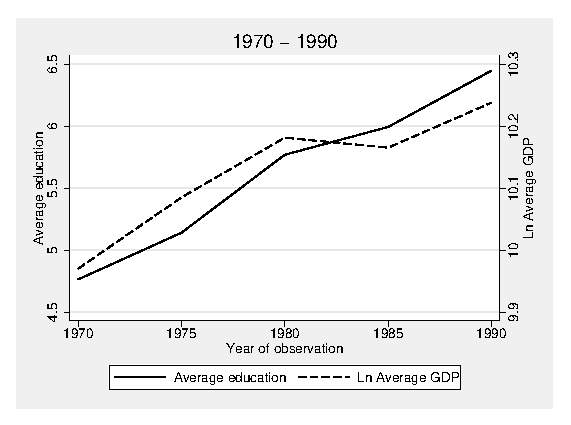
\includegraphics[scale=1.3]{graphs/mean_education_gdp_year.eps}
\caption{Education vs. GDP}
\label{fig:descriptives}
\end{figure}


\lipsum

Figure \ref{fig:descriptives} shows that...

\begin{table}[p]
	\caption{Regression results}
	\label{tab.r2}
			{
\def\sym#1{\ifmmode^{#1}\else\(^{#1}\)\fi}
\begin{tabular}{l*{5}{c}}
\hline\hline
            &\multicolumn{1}{c}{OLS}&\multicolumn{1}{c}{IV}&\multicolumn{1}{c}{FE}&\multicolumn{1}{c}{RE}&\multicolumn{1}{c}{FE (cluster)}\\
\hline
Education   &      0.2011\sym{***}&      0.2041\sym{***}&      0.0275         &      0.0551\sym{***}&     -0.0180         \\
            &      (0.02)         &      (0.02)         &      (0.02)         &      (0.02)         &      (0.04)         \\
[1em]
Log Capital &      0.1958\sym{***}&      0.1932\sym{***}&      0.2243\sym{***}&      0.1966\sym{***}&      0.2126\sym{***}\\
            &      (0.03)         &      (0.03)         &      (0.03)         &      (0.03)         &      (0.06)         \\
[1em]
Openness    &      0.0061\sym{***}&      0.0061\sym{***}&     -0.0020\sym{***}&     -0.0017\sym{***}&     -0.0020\sym{**} \\
            &      (0.00)         &      (0.00)         &      (0.00)         &      (0.00)         &      (0.00)         \\
\hline
\(N\)       &         232         &         232         &         232         &         232         &         232         \\
\textit{AIC}&    476.3275         &    476.3513         &    -3.2e+02         &           .         &    -3.2e+02         \\
Log likelihood&    -2.3e+02         &    -2.3e+02         &    162.1656         &                     &    165.2199         \\
$R^{2}$     &      0.5793         &      0.5793         &      0.4423         &                     &      0.4568         \\
F statistic (overall)&    104.6699         &    104.4600         &     48.1072         &                     &     27.6674         \\
Root MSE    &      0.6697         &      0.6639         &      0.1358         &      0.1440         &      0.1208         \\
\hline\hline
\multicolumn{6}{l}{\footnotesize Notes: standard errors in parenthesis. Significance levels: *, 10\%;}\\
\multicolumn{6}{l}{\footnotesize **, 5\%; ***, 1\%. The dependent variable is ln real GDP per workers.}\\
\multicolumn{6}{l}{\footnotesize Source: own computations.}\\
\end{tabular}
}

\end{table}


\lipsum

\begin{figure}[!htb]
\centering
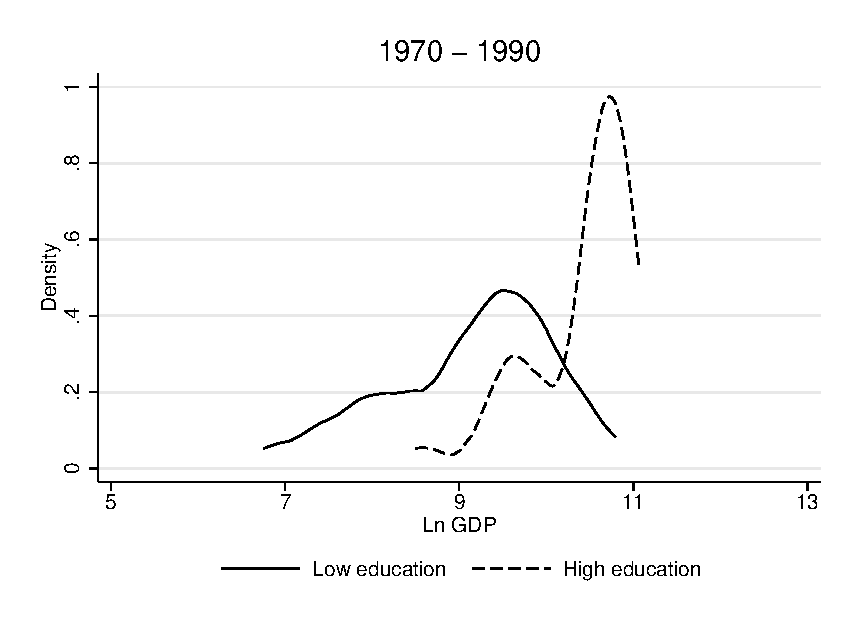
\includegraphics[scale=0.8]{graphs/lngdp_education.eps}
\caption{GDP distribution by level of education}
\label{fig:descriptives2}
\end{figure}

\lipsum

\section*{Appendix: number of observations by country}


\begin{table}[htbp]\centering 
\caption{\label{freq_cty_id} 
\textbf{Countries}}
\begin{tabular} {@{} l r r @{}} \\ \hline
Item& Number & Per cent \\
\hline
Afghanistan&        9&       11\\
Algeria&        9&       11\\
Argentina&        9&       11\\
Australia&        9&       11\\
Austria&        9&       11\\
Bahrain&        9&       11\\
Bangladesh&        9&       11\\
Barbados&        9&       11\\
Belgium&        9&       11\\
Belize&        3&        4\\
Total&       84&      100\\
\hline
\multicolumn{3}{@{}l}{\footnotesize{\emph{Source:} ../data/growthdata.dta}}
\end{tabular}
\end{table}






\end{document}
